\documentclass[tikz]{standalone}


\usepackage[cm]{sfmath}
\renewcommand{\familydefault}{\sfdefault}
\usepackage{sansmathaccent}

\usepackage{xcolor}

\usepackage{tikz}
\usetikzlibrary{backgrounds}

\definecolor{Dark2-A}{RGB}{ 27, 158, 119}
\definecolor{Dark2-B}{RGB}{217,  95,   2}

\definecolor{Set1-A}{RGB}{228,  26,  28}
\definecolor{Set1-B}{RGB}{ 55, 126, 184}

\tikzstyle{e}=[rounded corners,very thick,draw=white,double=black,arrows={-latex[black]}]
\tikzstyle{e-gray}=[e,draw=white,double=lightgray,arrows={-latex[lightgray]}]
\tikzset{every label/.style={rectangle,fill=none,draw=none, label distance=4pt}}

\tikzstyle{n}=[circle,fill=white,draw=white,line width=2pt,outer sep=0pt,inner sep=0pt, minimum size=4ex]
\tikzstyle{n square}=[n,rectangle,inner xsep=2pt,outer sep=2pt]

\tikzstyle{inline}=[anchor=base]
\tikzstyle{open}=[fill=Dark2-A!50]
\tikzstyle{closed}=[fill=Dark2-B!50]
\tikzstyle{conditioned}=[draw=black,line width=2pt]
\tikzstyle{unfair}=[text=Dark2-B]
\tikzstyle{bias}=[draw=Dark2-B]
\tikzstyle{unobserved}=[fill opacity=0.5]

\newcommand\innode[ 2 ]{ 
  \begin{tikzpicture}[baseline] 
      \node[inline,inner ysep=0pt,inner xsep=3pt,outer sep=0pt,opacity=0] (n) {#1}; 
      \useasboundingbox (n.north west) rectangle (n.south east);
      \node[n,minimum size=3ex,inner sep=1pt,inline,#2] {#1}; 
  \end{tikzpicture}
  }

\makeatletter
\DeclareRobustCommand{\rvdots}{%
  \vbox{
    \baselineskip4\p@\lineskiplimit\z@
    \kern-\p@
    \hbox{.}\hbox{.}\hbox{.}
  }}
\makeatother

\usetikzlibrary{calc}

\begin{document}
  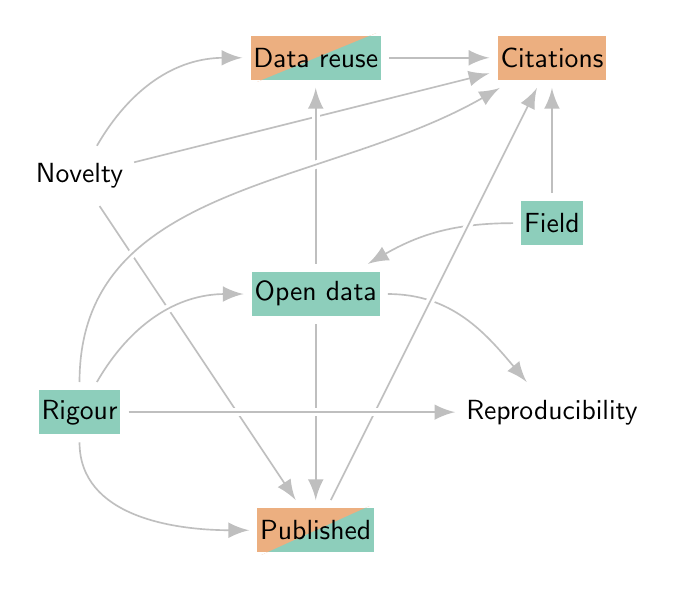
\begin{tikzpicture}[nodes=n square,
                      x=3cm,y=3cm]

    \begin{scope}[every edge/.style={e,double=lightgray,arrows={-latex[lightgray]}}]
        \tikzstyle{n-novelty}+=[]
        \tikzstyle{n-rigour}+=[open]
        \tikzstyle{n-data_reuse}+=[open]
        \tikzstyle{n-open_data}+=[open]

        \tikzstyle{n-published}+=[open]
        \tikzstyle{n-citations}+=[closed]
        \tikzstyle{n-reproducibility}+=[]
        \tikzstyle{n-field}+=[open]

        
    \node[n-novelty]         (novelty) at         (0, 1.5)         {Novelty};
    \node[n-rigour]          (rigour) at          (0, 0.5)          {Rigour};

    \node[n-data_reuse]      (data_reuse) at      (1, 2)        {Data reuse};
    \node[n-open_data]       (open_data) at       (1, 1)         {Open data};
    \node[n-published]       (published) at       (1, 0)         {Published};

    \node[n-citations]       (citations) at       (2, 2)         {Citations};
    \node[n-reproducibility] (reproducibility) at (2, 0.5) {Reproducibility};

    \node[n-field]           (field) at           (2, 1.3)           {Field};

    \draw[e,->]
      (data_reuse) edge (citations)
      (field)      edge (citations)
      (field)      edge[out=180,in=30] (open_data)
      (novelty)    edge (citations)
      (novelty)    edge[out=60,in=180] (data_reuse)
      (novelty)    edge (published)
      (open_data)  edge (data_reuse)
      (open_data)  edge (published)
      (open_data)  edge[out=0,in=130] (reproducibility)
      (published)  edge (citations)
      (rigour)     edge[out=90,in=210] (citations)
      (rigour)     edge[out=60,in=180] (open_data)
      (rigour)     edge[out=-90,in=180] (published)
      (rigour)     edge (reproducibility);


        \begin{scope}
            \clip (published.south west) -- (published.north east) -- (published.north west) -- cycle;
            \node[closed] () at (published) {Published};
        \end{scope}

        \begin{scope}
            \clip (data_reuse.south west) -- (data_reuse.north east) -- (data_reuse.north west) -- cycle;
            \node[closed] () at (data_reuse) {Data reuse};
        \end{scope}

    \end{scope}

  \end{tikzpicture}
\end{document}